\section{Projekt Infrastruktury Sieciowej}

\subsection{Schemat logiczny sieci}
        
    \begin{figure}[!htb]
        \centering
        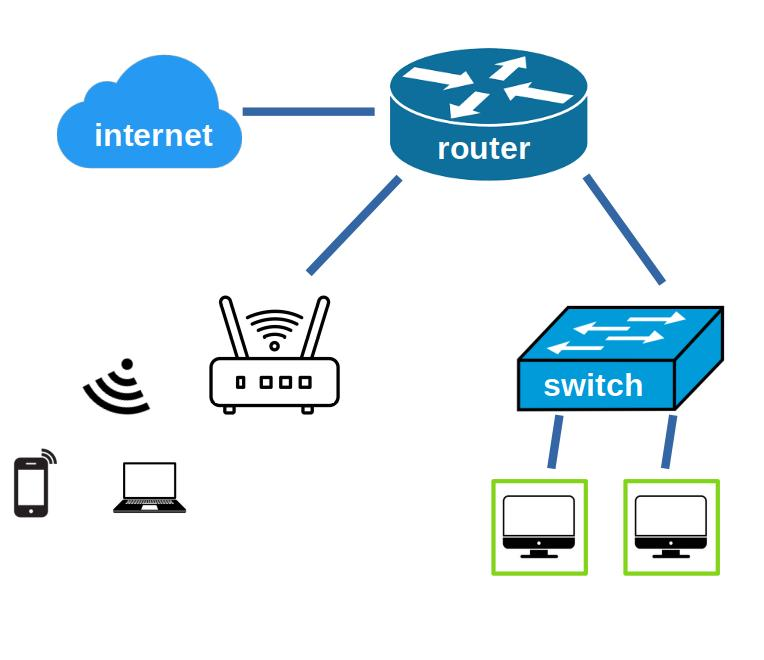
\includegraphics[width=0.6\textwidth]{schematy/logiczny}
        \caption{Schemat logiczny sieci}
    \end{figure}

\subsection{Schemat poprowadzenia okablowania}




    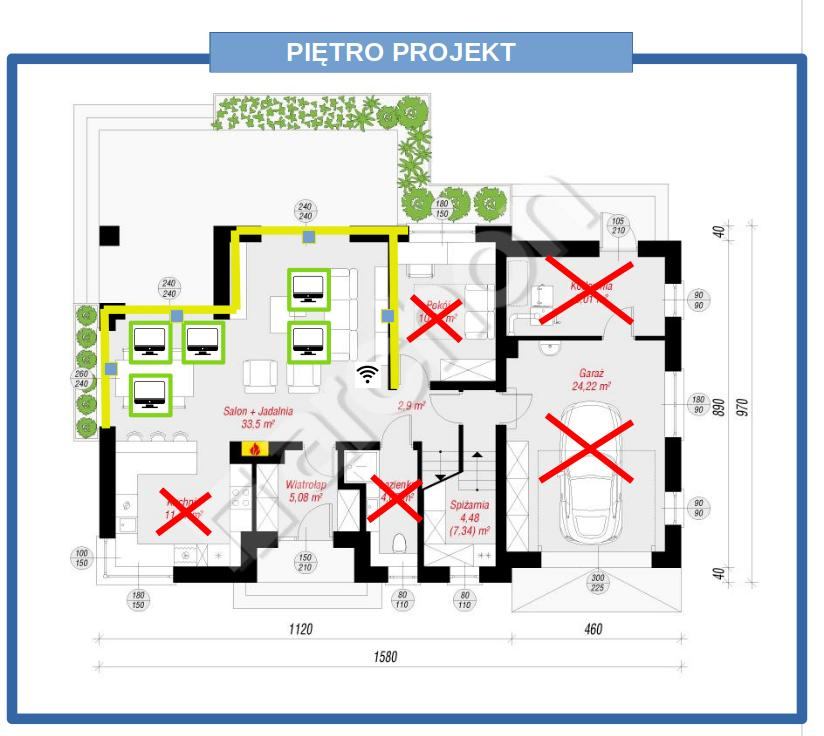
\includegraphics[width=0.9\textwidth]{projekty/parter}


    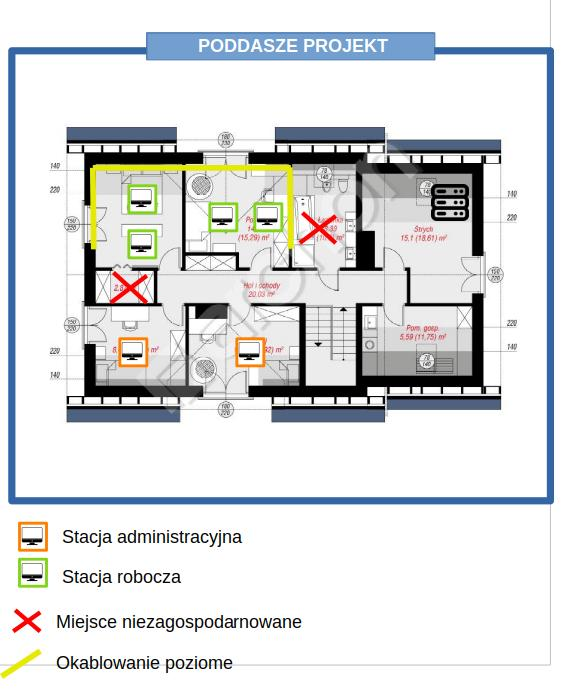
\includegraphics[width=0.9\textwidth]{projekty/poddasze}


\pagebreak

\subsection{Topologia Sieci}

    W projekcie infrastruktury sieciowej firmy XYZ proponujemy zastosowanie topologii sieci opartej na modelu gwiazdy. Każde stanowisko komputerowe, w tym stacje robocze i stacje administracyjne, będzie podłączone bezpośrednio do centralnego przełącznika (switcha). To rozwiązanie zapewnia prostą skalowalność i łatwe zarządzanie siecią.

        
    \begin{figure}[!htb]
        \centering
        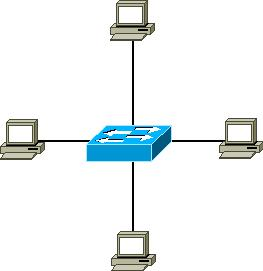
\includegraphics[width=0.3\textwidth]{gwiazda}
        \caption{Topologia Gwiazdy}
    \end{figure}

\subsection{Adresacja Sieci}

Sieć działa w jednej podsieci – 192.168.0.0/24, w której do dyspozycji przyznano następujące adresy:

\begin{itemize}
    \item Router – 192.168.0.1
    \item Switch – 192.168.0.2
    \item Stacje robocze – 192.168.0.10 – 192.168.0.32
    \item Access Point – 192.168.0.40
    \item o Wszelkie urządzenia otrzymują ustawienia z serwera DHCP w zakresie 192.168.0.50 –
    192.168.0.100
\end{itemize}



\subsection{Kable i Media Transmisyjne}

    Do połączenia urządzeń w sieci użyjemy kabli UTP kategorii 6 o odpowiedniej długości. Ponadto, w niektórych przypadkach zastosujemy kable światłowodowe, zwłaszcza tam, gdzie potrzebna jest duża przepustowość, na przykład między centralnym serwerem zasobów a głównym switchem.

\subsection{Urządzenia Sieciowe}
    W naszym projekcie użyjemy następujących urządzeń sieciowych:
    \begin{itemize}
        \item - Centralny przełącznik (switch) do obsługi wszystkich stanowisk.
        \item Router zapewniający dostęp do internetu oraz segregację sieci wewnętrznej i sieci gości.
        \item Access Pointy Wi-Fi dla zapewnienia dostępu do sieci bezprzewodowej.
        \item Firewall do zabezpieczenia sieci przed nieautoryzowanym dostępem.
    \end{itemize}



\subsection{Zapotrzebowanie na Przepustowość}

    Na podstawie analizy potrzeb firmy określiliśmy zapotrzebowanie na przepustowość sieci. Oceniliśmy, że przepustowość 1 GbE (Gigabit Ethernet) będzie wystarczająca dla stanowisk komputerowych, biorąc pod uwagę typowe obciążenia sieciowe w firmie.

\subsection{System Monitoringu i Bezpieczeństwa}

    W ramach zapewnienia bezpieczeństwa sieci, zainstalujemy system monitoringu sieciowego, który pozwoli na śledzenie aktywności sieciowej, wykrywanie nieautoryzowanych dostępów i reagowanie na potencjalne zagrożenia. Wprowadzimy również środki bezpieczeństwa, takie jak zapory ogniowe (firewalle) i systemy antywirusowe, aby chronić sieć przed atakami i złośliwym oprogramowaniem.

\subsection{Centralny punkt dystrybucyjny}
